\chapter{Introduction}
\label{chp:introduction}
Nowadays, 19\% of the global energy consumption is used for lighting. For this reason, saving energy in lighting is vital. A simple way to save energy is to “simply” turn the lights off, or reduce the amount of light used when nobody is around. This thesis proposes a new method for luminaires to detect the presence of humans and objects, namely \textit{Dark Sensing}.

The idea of human sensing is not new. Everybody in the western world has walked into a room where the lights suddenly turned on once they entered. The most common method to create this effect is to make use of a PIR (passive-infrared) sensor. By monitoring the infra-red radiation (heat) in the area, it can detect changes in the environment and toggle the light based on these changes. This method works very well but has several drawbacks. The first is that it's unable to detect objects with the same surface temperature as the environment, for example a car where the engine has just been turned on. Another drawback is that the PIR method has no potential for communication without the addition of extra components. Dark sensing attempts to overcome these drawbacks by only using a photodiode and the light in the visible spectrum a luminaire normally emits.

This thesis explores the idea of detecting changes in the environment with reflections of visible light. The proposed system works in the following manner: If nothing is in the area, the light will be turned on, but outputting a very low light level. Some of the light will reflect off the environment back to the light source. This can be measured with the photodiode. The signal received is a measure of the illuminated area. If something were to change in that area, a car drives by for example, then the reflections in the environment will change and therefore the light perceived by the photodiode will change as well. These changes will then result in a detection by the system which will turn the light on at full brightness. An overview of the scenario can be seen in \ref{fig:Introduction}.

\begin{figure}[]
	\centering     %%% not \center
	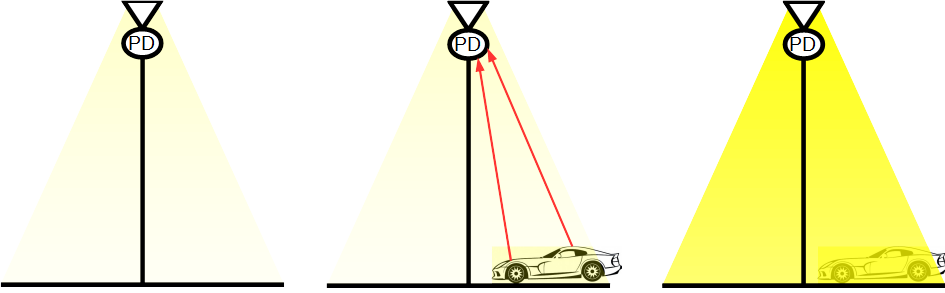
\includegraphics[width=120mm]{pics/SystemScenario.png}
	\caption{When no object is in the area, the luminaire will barely generate any light. If an object drives into the area, the reflections will be picked up by the photodiode, which will then turn the light on. \label{fig:Introduction}}
\end{figure}
The ultimate goal of the proposed system is to reduce the time the light needs to be on the nearly zero. This will lead to a light which barely consumes any energy while nobody is around but is still able to detect people, cars or other objects passing by. It might even be possible to decrease the light output to an amount which is invisible to the human eye, resulting in an unnoticeable, activity detecting, energy-saving device.

\section{Problem statement}
\label{Problem statement}
\textbf{Is it possible to create a system which can detect the activity of humans or objects by measuring reflections of visible light while being invisible to the human eye?}
\\
\\
This problem can be divided into three sub-questions:
\begin{itemize}\itemsep2pt
	\item How strong is a reflection obtained from a flash in a realistic scenario and how much does this reflection change if an object enters the area?
	\item What are the challenges in obtaining reflections when using a low-intensity light and how can they be tackled?
	\item What additional signals are received by the system (noise) and what algorithm can be used to convert the received signal in a reliable logical signal: Detection or no detection?
\end{itemize}

\section{Contributions}
\label{sec:Contributions}
This thesis proposes \textbf{Dark Sensing}, a system that uses reflections of an LED controlled with a low duty cycle (4\%), and therefore nearly invisible to the human eye, to detect changes in the surrounding area.
\begin{itemize}\itemsep2pt
	\item A model, estimating the change in signal (reflected light) when a object moves under, leaves or passes by the LED in different environments.
	\item A method to convert a captured reflection of the LED into a usable measure of the environment.
	\item An algorithm which analyses features of consecutive flashes and is capable of detecting objects moving under, leaving or passing through the illuminated area.
	\item A prototype capable of detecting between 73\% and 90\% of all humans passing by in a realistic environment dependent on the allowed false positive ratio (0 - 5\%).
\end{itemize}

\section{Organisation}
This thesis describes the development path of the new technique "Dark Sensing" from idea to a working prototype. Chapter 2 will present the required background knowledge to understand several choices made in this thesis and present the related work. In chapter 3 a model will be presented, which calculates the theoretical response of bypassing objects. Chapter 4 describes the created experimentation platform. Chapter 5 will focus on finding the ideal settings for generating an analysable flash and will explain what the best method is for extracting data from this flash. Chapter 6 explores the possibilities for analysing sets of consecutive flashes and proposes an algorithm to detect significant changes in the signal. Chapter 7 tests the prototype created and evaluates the performance of system. The thesis concludes with an evaluation of the new "Dark Sensing" technology and suggests several possible directions for future work.